%==============================================================================
% Chapitre 46 - Le calibre
%==============================================================================

\section{Introduction}

Le terme \emph{calibre} est probablement l'un des plus connus dans le domaine
des armes à feu.

Il est pourtant souvent utilisé pour désigner des réalités différentes selon
le contexte.

Le calibre peut en effet faire référence :

\begin{itemize}
    \item au diamètre du projectile ;
    \item au diamètre du canon ;
    \item à une famille de cartouches ;
    \item à une désignation commerciale.
\end{itemize}

Cette diversité d'usages est source de nombreuses confusions.

\begin{aretenir}

Le terme calibre ne possède pas toujours une signification unique.

\end{aretenir}

\section{Définition générale}

Dans son sens le plus courant, le calibre correspond à une dimension
caractéristique liée au diamètre.

Dans les armes à feu, il est généralement exprimé :

\begin{itemize}
    \item en millimètres ;
    \item en fractions de pouce ;
    \item plus rarement sous d'autres formes historiques.
\end{itemize}

\section{Calibre du projectile}

Le calibre peut désigner le diamètre du projectile.

Par exemple :

\begin{itemize}
    \item un projectile de 9 mm possède un diamètre voisin de 9 mm ;
    \item un projectile de .308 pouce possède un diamètre voisin de
          7,82 mm.
\end{itemize}

Cette définition semble simple mais n'est pas toujours suffisante.

\section{Calibre du canon}

Le calibre peut également désigner une dimension du canon.

Or plusieurs méthodes de mesure existent.

Selon les pays et les époques, la mesure peut être réalisée :

\begin{itemize}
    \item entre les sommets des rayures ;
    \item entre les fonds des rayures.
\end{itemize}

Cette différence explique certaines incohérences apparentes.

\section{Les rayures du canon}

Dans un canon rayé, deux diamètres principaux peuvent être définis :

\begin{itemize}
    \item le diamètre entre les sommets des rayures ;
    \item le diamètre entre les fonds des rayures.
\end{itemize}

Le projectile possède généralement un diamètre proche du diamètre à fond de
rayures.



\begin{figure}[htbp]
\centering

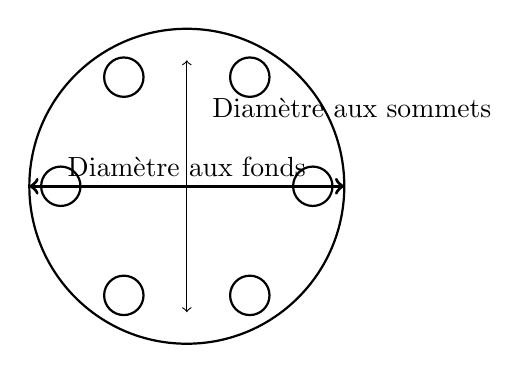
\begin{tikzpicture}[scale=1]

% Fond de rayures
\draw[thick] (0,0) circle (2);

% Sommets
\foreach \a in {0,60,120,180,240,300}
{
    \draw[thick]
    ({1.6*cos(\a)},{1.6*sin(\a)})
    circle (0.25);
}


% Diamètre aux fonds
\draw[<->,very thick]
(-2,0)
--
(2,0);

\node[above]
at (0,0)
{Diamètre aux fonds};

% Diamètre aux sommets
\draw[<->]
(0,-1.6)
--
(0,1.6);

\node[right]
at (0.2,1.0)
{Diamètre aux sommets};

\end{tikzpicture}

\caption{Diamètre aux sommets et diamètre aux fonds des rayures.}
\label{fig:rayures_coupe}

\end{figure}

\section{Exemple du .308 Winchester}

Le .308 Winchester constitue un exemple classique.

Son projectile présente un diamètre nominal de :

\begin{equation}
0,308~\text{pouce}
\end{equation}

soit environ :

\begin{equation}
7,82~\text{mm}
\end{equation}

Pourtant, sa désignation ne fournit aucune information sur la longueur de
l'étui ou les autres caractéristiques de la cartouche.

\section{Millimètres et pouces}

Deux systèmes d'unités coexistent largement :

\begin{itemize}
    \item le système métrique ;
    \item le système impérial.
\end{itemize}

On rencontre ainsi des désignations telles que :

\begin{itemize}
    \item 9 mm ;
    \item 7,62 mm ;
    \item .22 ;
    \item .30 ;
    \item .45.
\end{itemize}

\section{Conversion}

La relation entre pouce et millimètre est :

\begin{equation}
1~\text{pouce}=25,4~\text{mm}
\end{equation}

Cette conversion permet de comparer les différentes désignations.

\section{Des désignations parfois trompeuses}

Certaines appellations historiques ne correspondent pas exactement au
diamètre réel du projectile.

Les raisons sont diverses :

\begin{itemize}
    \item traditions industrielles ;
    \item héritage historique ;
    \item évolutions techniques ;
    \item considérations commerciales.
\end{itemize}

Le calibre indiqué doit donc être considéré comme une désignation plutôt que
comme une mesure exacte.

\section{Familles de calibres}

Plusieurs cartouches peuvent utiliser des projectiles de diamètre voisin.

Par exemple, de nombreuses cartouches utilisent des projectiles de :

\begin{equation}
0,308~\text{pouce}
\end{equation}

tout en présentant des performances très différentes.

\section{Petit calibre et gros calibre}

Les notions de petit et gros calibre dépendent fortement du contexte.

Dans les armes légères, on considère souvent :

\begin{itemize}
    \item les petits calibres ;
    \item les calibres intermédiaires ;
    \item les gros calibres.
\end{itemize}

Ces catégories ne possèdent toutefois pas de limites universelles.

\section{Le cas de l'artillerie}

Dans le domaine de l'artillerie, le calibre désigne généralement le diamètre
intérieur du tube.

On rencontre ainsi :

\begin{itemize}
    \item 105 mm ;
    \item 120 mm ;
    \item 155 mm.
\end{itemize}

\section{Calibre et longueur du tube}

Pour certaines armes, le calibre est également utilisé comme unité de
longueur.

Une pièce d'artillerie peut par exemple être décrite comme :

\begin{quote}
155 mm L/52
\end{quote}

Cela signifie que la longueur du tube vaut 52 fois son calibre.

\begin{figure}[htbp]
\centering

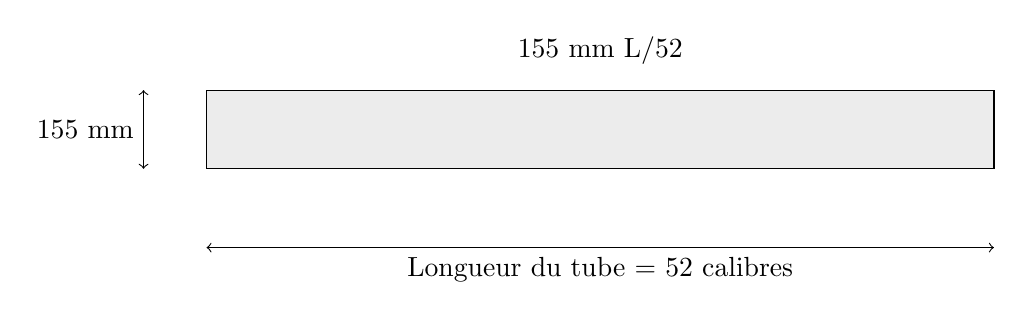
\begin{tikzpicture}[scale=1]

% Tube
\draw[fill=gray!15]
(0,0)
rectangle
(10,1);

% Bouche
\draw[thick]
(10,0)
--
(10,1);

% Calibre
\draw[<->]
(-0.8,0)
--
(-0.8,1);

\node[left]
at (-0.8,0.5)
{155 mm};

% Longueur
\draw[<->]
(0,-1)
--
(10,-1);

\node[below]
at (5,-1)
{Longueur du tube = 52 calibres};

\node[above]
at (5,1.2)
{155 mm L/52};

\end{tikzpicture}

\caption{Exemple de désignation d'une pièce d'artillerie de type 155 mm L/52.}
\label{fig:l52}

\end{figure}

\section{Exemple}

Pour une pièce de :

\begin{equation}
155~\text{mm}
\end{equation}

et :

\begin{equation}
L/52
\end{equation}

la longueur du tube est :

\begin{equation}
155\times52
=
8060~\text{mm}
\end{equation}

soit environ :

\begin{equation}
8,06~\text{m}
\end{equation}

\section{Calibre et performances}

Le calibre influence notamment :

\begin{itemize}
    \item la masse du projectile ;
    \item la quantité d'énergie transportée ;
    \item le recul ;
    \item les effets terminaux.
\end{itemize}

Cependant, le calibre seul ne permet pas de prédire les performances d'une
munition.

\section{Pourquoi le calibre ne suffit pas}

Deux cartouches de même calibre peuvent présenter :

\begin{itemize}
    \item des masses de projectile différentes ;
    \item des vitesses différentes ;
    \item des pressions différentes ;
    \item des énergies très différentes.
\end{itemize}

La désignation complète de la cartouche reste donc indispensable.

\section{Vers les désignations de cartouches}

Le calibre constitue seulement une partie de l'identité d'une munition.

Pour distinguer précisément les nombreuses cartouches existantes, des
systèmes de désignation plus complets ont été développés.

Ils feront l'objet du chapitre suivant.

\section{À retenir}

\begin{aretenir}

\begin{itemize}
    \item Le calibre est généralement lié à une notion de diamètre.
    \item Il peut désigner le projectile, le canon ou une famille de
          cartouches.
    \item Les désignations ne correspondent pas toujours exactement aux
          dimensions réelles.
    \item Deux cartouches de même calibre peuvent avoir des performances très
          différentes.
    \item Le calibre seul ne suffit pas à identifier une munition.
\end{itemize}

\end{aretenir}
